\begin{figure}[htbp]
\centering
% Figure7.jpg and Figure8.jpg are JPEG copies (quality 90) of the hardware
% photographs, Figure7 resized to 1200 px wide; the originals are kept out of
% the repository (see README). Nothing else is edited. Native clipping only
% enlarges the contact region in the three original bottom-row hardware frames.
\begin{tikzpicture}[paperfigure]
  \path[use as bounding box] (0,0) rectangle (15.3,5.05);
  \node[paneltitle] at (0,4.85) {(a) Experimental setup};
  \node[anchor=south west,inner sep=0] at (0,0)
    {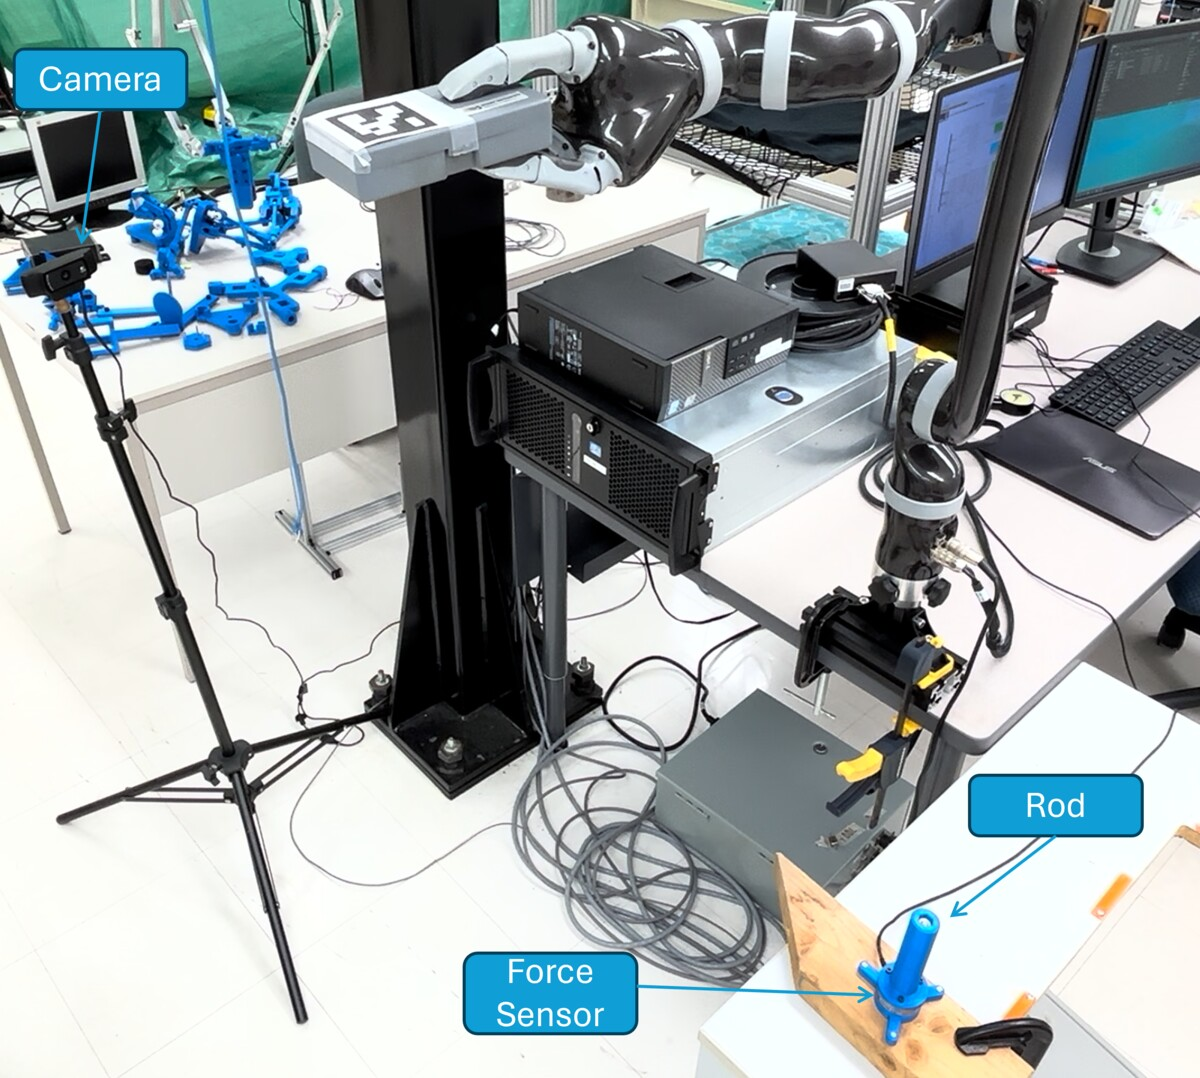
\includegraphics[width=5.1cm]{Figure7.jpg}};
  \node[paneltitle] at (6.0,4.85) {(b) MuJoCo sequence};
  \node[anchor=south west,inner sep=0] at (6.0,.95)
    {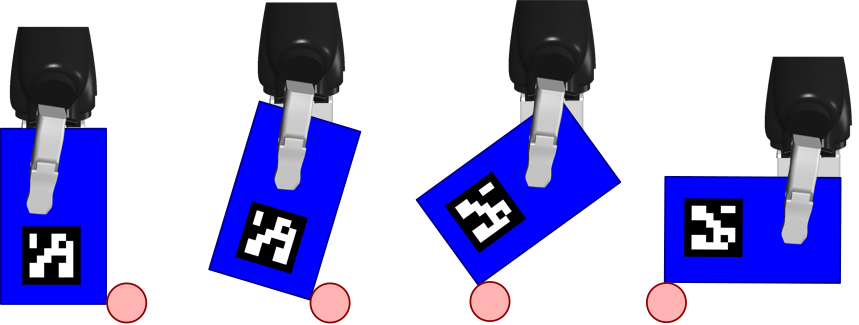
\includegraphics[width=8.4cm]{Figure6.png}};
  \foreach \x/\stage in {6.84/1,8.87/2,11.18/3,13.59/4} {
    \draw[motion,line width=1.1pt] (\x,3.95) -- ++(.385,0);
    \node[anchor=north] at (\x+.15,.85) {Stage \stage};
  }
  \node[anchor=west] at (6.0,.1) {Parallel arrows: fixed wrist orientation};
\end{tikzpicture}

\vspace{2mm}
\begin{tikzpicture}[paperfigure]
  \path[use as bounding box] (0,-.55) rectangle (15.3,5.1);
  \node[paneltitle] at (0,4.92) {(c) Hardware contact region};
  % Figure8.jpg is 3033 by 1819 pixels. Its three bottom frames
  % have equal widths. Identical lower-right regions are shown at the same scale.
  \foreach \x/\sx/\stage in {
    0/-5.5/{Approach / contact},
    5.3/-15.61/{Intermediate},
    10.6/-25.72/{Final}}
  {
    \begin{scope}[shift={(\x,0)}]
      \clip (0,0) rectangle (4.61,4.595);
      \node[anchor=south west,inner sep=0] at (\sx,0)
        {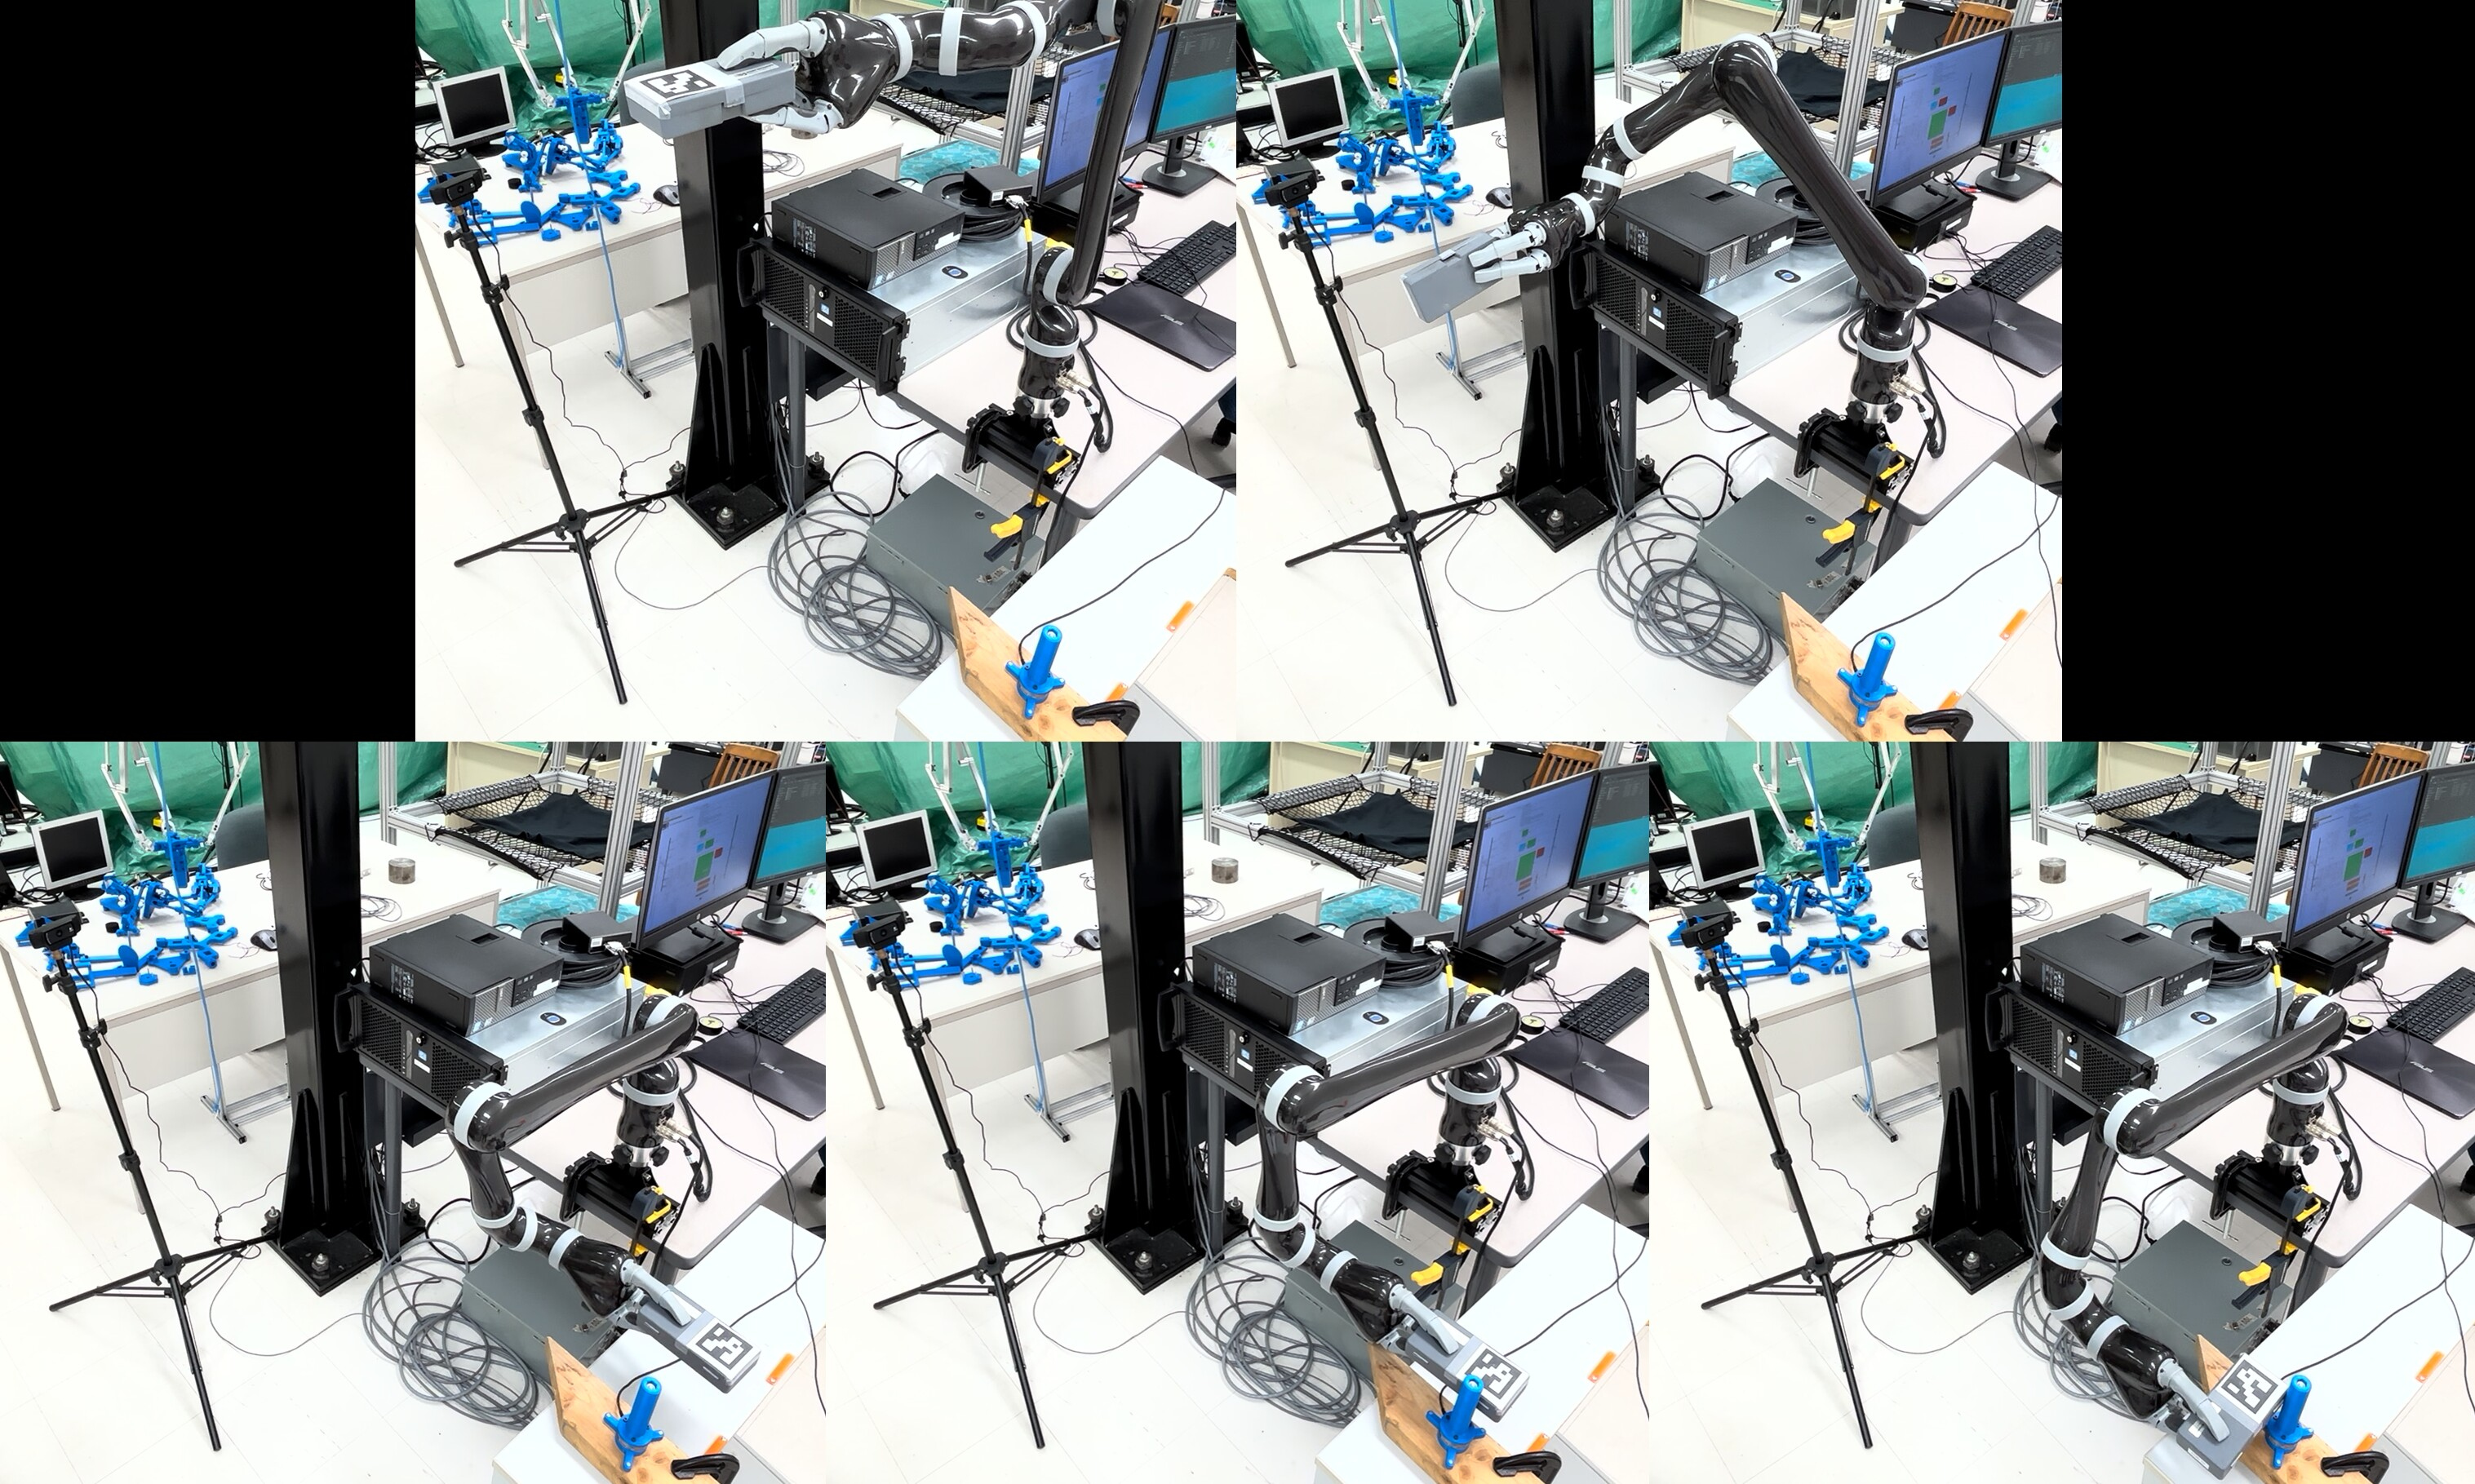
\includegraphics[width=30.33cm]{Figure8.jpg}};
    \end{scope}
    \node[anchor=north,text width=4.61cm,align=center] at (\x+2.305,-.1) {\stage};
  }
\end{tikzpicture}
\caption{Original setup and MuJoCo sequence, with three enlarged hardware contact-region crops in their original order. Stage labels carry no measured timestamps or angles.}
\label{fig:experiment_setup}
\end{figure}
